\documentclass[journal,10pt,twocolumn]{IEEEtran}

\usepackage{cite}
\usepackage{graphicx}
\usepackage{amsmath,amssymb,amsfonts}
\usepackage{textcomp}
\usepackage{xcolor}
\usepackage{xurl}
\usepackage{microtype}
\usepackage[colorlinks=false, hidelinks]{hyperref}

\hyphenation{op-tical net-works semi-conduc-tor to-ken-i-za-tion}

% =========================================================
\begin{document}
% =========================================================

\title{Beyond $T+2$: On-Chain Regulatory Enforcement for Institutional Real-World Asset Tokenization}

\author{%
\begin{minipage}[t]{0.46\linewidth}
  \centering
  Zakaria Rahali\\[3pt]
  {\small\itshape Cybersecurity and Network Infrastructures\\
  Moroccan School of Engineering Sciences -- EMSI\\
  Rabat 10000, Morocco\\}
  {\small\upshape\href{mailto:zakaria.rahali@emsi-edu.ma}{zakaria.rahali@emsi-edu.ma}}
\end{minipage}%
\hfill%
\begin{minipage}[t]{0.46\linewidth}
  \centering
  Author Three\\[3pt]
  {\small\itshape Department\\
  Institution\\
  City, Country\\}
  {\small\upshape email@domain.com}
\end{minipage}\\[4ex]
\begin{minipage}[t]{0.46\linewidth}
  \centering
  Aya Belkhaouad\\[3pt]
  {\small\itshape Cybersecurity and Network Infrastructures\\
  Moroccan School of Engineering Sciences -- EMSI\\
  Rabat 10000, Morocco\\}
  {\small\upshape\href{mailto:aya.belkhaouad@emsi-edu.ma}{aya.belkhaouad@emsi-edu.ma}}
\end{minipage}%
\hfill%
\begin{minipage}[t]{0.46\linewidth}
  \centering
  Author Four\\[3pt]
  {\small\itshape Department\\
  Institution\\
  City, Country\\}
  {\small\upshape email@domain.com}
\end{minipage}%
\thanks{This research forms the architectural blueprint of the ``Blockchain: Real-World Asset Tokenization Platform'' project, demonstrating the integration of traditional finance compliance mechanisms within distributed ledger technology. Manuscript submitted April 2026.}}

\markboth{\textls[180]{Institutional Tokenization\ \ \textperiodcentered\ \ April 2026}}%
{Rahali and Belkhaouad: Beyond $T+2$ — On-Chain Regulatory Enforcement}

\maketitle

% =========================================================
\begin{abstract}
% =========================================================
Traditional securities settlement currently requires $T+2$ or $T+3$ days, trapping an estimated \$10 trillion in collateral globally and generating systemic counterparty risk \cite{ref:rwa_fsb}. The tokenization of Real-World Assets (RWA) on distributed ledgers promises to resolve these inefficiencies, yet institutional adoption is constrained by a fundamental regulatory incompatibility: public blockchains cannot natively enforce Know Your Customer (KYC), Anti-Money Laundering (AML), or the Markets in Crypto-Assets (MiCA) regulation.

In this paper, we introduce the \textit{Regulatory-Embedded Consensus} (REC) model, a formally specified architecture built on Hyperledger Fabric. Unlike prior approaches that relegate regulators to passive auditor nodes, REC elevates the regulatory authority $\mathcal{R}$ to an active, endorsing participant whose cryptographic signature is a prerequisite for any state transition. We prove that REC satisfies both \textit{safety} (no non-compliant transaction can be committed) and \textit{liveness} (compliant transactions are always eventually committed) under a non-colluding adversary model.

Our model enforces ISIN, LEI, and ISO~4217 validations on-chain and natively implements MiCA Article~68 threshold reporting. Off-chain AML analysis is orchestrated via a graph database, achieving pre-submission fraud screening with an overhead of 50--100\,ms per transaction. Simulation-based projections indicate sustained throughput of 950--1,350 TPS under the dual-endorser policy, exceeding the requirements of institutional RWA settlement by two orders of magnitude. We present a formal model, a comparative analysis against six distributed ledger paradigms, an end-to-end asset lifecycle, a theoretical architecture, and a STRIDE-based threat model.
\end{abstract}

\begin{IEEEkeywords}
Real-World Assets (RWA), Tokenization, Hyperledger Fabric, Distributed Ledger Technology, Regulatory Compliance, MiCA, Regulatory-Embedded Consensus (REC), KYC/AML, Permissioned Blockchain, Smart Contracts.
\end{IEEEkeywords}

% =========================================================
\section{Introduction}
\label{sec:intro}
% =========================================================

\IEEEPARstart{T}{raditional} financial markets are burdened by deeply entrenched structural inefficiencies. The settlement of securities and illiquid assets under the prevailing $T+2$ or $T+3$ cycle traps an estimated \$10 trillion in collateral globally, imposes bilateral counterparty credit risk, and generates operational overhead that consumes an estimated 10\% of post-trade revenue \cite{ref:rwa_fsb, ref:ecb_dlt}. The Bank for International Settlements (BIS) identifies settlement latency as one of the principal systemic vulnerabilities in modern capital markets \cite{ref:bis_tokenisation}.

The tokenization of Real-World Assets (RWA), defined as the process of representing ownership rights to physical or financial assets as programmable tokens on a distributed ledger, promises to fundamentally resolve these inefficiencies. By encoding asset semantics directly in smart contracts, tokenization enables atomic delivery-versus-payment (DvP), programmable fractional ownership, and automated corporate actions such as dividend distributions and covenant enforcement, all executed with deterministic, sub-second finality \cite{ref:setl2023}.

Despite these theoretical advantages, institutional adoption has largely stalled for three compounding reasons. First, public, permissionless blockchains such as Ethereum expose transaction graphs pseudonymously, creating irreconcilable conflicts with client data privacy mandates under GDPR and MiFID~II. Second, probabilistic consensus mechanisms (Proof-of-Work or Proof-of-Stake) cannot provide the settlement finality guarantee required by central counterparties (CCPs). Third, and most critically, the European Union's Markets in Crypto-Assets (MiCA) regulation \cite{ref:mica} and the FATF Recommendation~16 for virtual asset service providers \cite{ref:fatf} impose strict reporting, governance, and transaction monitoring obligations that anonymous on-chain participants are structurally incapable of fulfilling.

Existing permissioned blockchain solutions partially address these concerns. Hyperledger Fabric \cite{ref:fabric} provides channel-based privacy and pluggable endorsement policies but, in standard deployments, assigns regulators to passive auditor roles. R3 Corda \cite{ref:corda} achieves bilateral privacy through point-to-point transaction flows but lacks a global shared state, hindering systemic surveillance. DAML \cite{ref:daml} provides a high-level smart contract language with privacy primitives but does not natively embed regulatory endorsement in the consensus path.

This paper makes four principal contributions. We formalize the Regulatory-Embedded Consensus (REC) model by defining a tuple of actors and a strict endorsement policy that elevates the regulatory authority to an active consensus participant. We then prove that REC satisfies both safety and liveness under a standard non-colluding adversary model. We further describe a conceptual architecture based on Hyperledger Fabric that integrates off-chain AML analysis and secure identity management. Finally, we present a simulation-based performance evaluation alongside a STRIDE-based threat model that collectively characterize the security posture and operational viability of the proposed architecture.

The remainder of this paper is organized as follows. Section~\ref{sec:related} surveys related work. Section~\ref{sec:rec} formalizes the REC model. Section~\ref{sec:comparison} presents a comparative analysis. Section~\ref{sec:arch} describes the theoretical architecture. Section~\ref{sec:usecase} traces an end-to-end asset lifecycle. Section~\ref{sec:perf} evaluates performance. Section~\ref{sec:threat} presents the threat model. Section~\ref{sec:limits} discusses limitations. Section~\ref{sec:conclusion} concludes.

% =========================================================
\section{Related Work}
\label{sec:related}
% =========================================================

\subsection{Permissioned Blockchain Platforms}

Androulaki \textit{et al.} \cite{ref:fabric} introduced Hyperledger Fabric as a modular, permissioned blockchain operating system. Its execute-order-validate (EOV) pipeline decouples transaction simulation from consensus ordering, enabling throughputs exceeding 3,000 TPS in controlled environments \cite{ref:manevich}. However, standard Fabric deployments assign regulatory entities as channel members with read access only; they do not participate in the endorsement policy, meaning compliance validation occurs off-chain at best.

R3 Corda \cite{ref:corda} was designed explicitly for financial institutions and uses a notary-based finality model with point-to-point data sharing. While Corda achieves strong bilateral privacy, its absence of a global shared ledger complicates holistic regulatory surveillance. The DAML smart contract language \cite{ref:daml} adds a privacy-preserving execution model atop distributed ledgers, but its compliance enforcement relies on off-chain legal interpretation rather than on-chain cryptographic guarantees.

The ConsenSys Quorum platform (now Hyperledger Besu) \cite{ref:quorum} provides an Ethereum-compatible permissioned environment with private transaction groups. However, it inherits Ethereum's gas-based execution model and its compliance enforcement remains programmatic rather than structurally embedded in the consensus layer.

\subsection{Regulatory Compliance on Distributed Ledgers}

Garg \textit{et al.} \cite{ref:garg2021} survey on-chain KYC approaches across Fabric, Ethereum, and Corda, concluding that no existing platform natively enforces regulator-in-the-loop transaction validation. A regulator-as-endorser design is identified as an open research direction.

Wüst and Gervais \cite{ref:wust2018} provide a formal decision framework for choosing blockchain architectures, noting that permissioned ledgers are strictly preferable for regulated financial applications due to finality guarantees, but do not address how regulators can be embedded in the consensus protocol itself.

The European Central Bank's DLT pilot \cite{ref:ecb_dlt} experimented with central bank money settlement on permissioned ledgers and found that regulator participation as a passive observer was insufficient for real-time systemic risk monitoring, motivating the need for active regulator integration.

\subsection{RWA Tokenization Platforms}

The FSB \cite{ref:rwa_fsb} identifies the primary barriers to institutional RWA tokenization as the lack of standardized on-chain legal representations, the inability to enforce AML/KYC natively, and interoperability gaps between tokenized and traditional settlement infrastructure. The BIS \cite{ref:bis_tokenisation} further notes that private ledgers with embedded regulatory logic represent the most viable near-term path for institutional adoption.

Setl \textit{et al.} \cite{ref:setl2023} implement a Fabric-based tokenization platform for equities but rely on an off-chain compliance engine. Their reported latency of 150--200\,ms per transaction demonstrates the feasibility of permissioned ledgers for institutional use but does not address the oracle dependency problem created by off-chain AML systems.

\subsection{Gap Analysis}

Across the literature surveyed, no prior work formalizes a consensus model in which a regulatory authority holds an active cryptographic endorsement role as a structural invariant of the protocol. Prior approaches either assign regulators to passive observer roles, perform compliance validation off-chain without on-chain enforcement, or rely on programmatic smart contract logic that can be bypassed by consortium administrators with sufficient access. REC addresses all three gaps by making regulatory endorsement a protocol-level prerequisite for state commitment.

% =========================================================
\section{The Regulatory-Embedded Consensus (REC) Model}
\label{sec:rec}
% =========================================================

In public blockchains, the consensus mechanism solely verifies cryptographic signatures and prevents double-spending. In our architecture, consensus is expanded to inherently guarantee deterministic regulatory compliance before any state transition is committed.

\subsection{Actor Model}

The REC network $\mathcal{N}$ is defined by the tuple $\mathcal{N} = \langle \mathcal{F}, \mathcal{R}, \mathcal{O} \rangle$, where $\mathcal{F}$ is the set of Financial Operators (e.g., commercial banks), each operating one or more endorsing peer nodes responsible for asset origination, client onboarding, and transaction proposal submission; $\mathcal{R}$ is the set of Regulatory Bodies (e.g., the AMF), each operating an independent endorsing peer node executing compliance validation functions; and $\mathcal{O}$ is the Ordering Service, an EtcdRaft cluster responsible for deterministic transaction sequencing and crash fault-tolerant (CFT) finality.

\subsection{Formal Endorsement Policy}

Let $\mathcal{T}$ be a proposed transaction (e.g., \texttt{TransferAsset}). Let $V_{state}(\mathcal{T})$ denote the standard world-state validity function and $V_{comp}(\mathcal{T})$ denote a compliance validation function executed exclusively by $\mathcal{R}$, evaluating KYC status, AML flags, sanction list membership, and MiCA threshold constraints. The REC endorsement policy $\mathbb{E}$ holds that a transaction $\mathcal{T}$ reaches committed state if and only if it carries valid cryptographic signatures from both $\mathcal{F}$ and $\mathcal{R}$:
\begin{equation*}
\mathbb{E}(\mathcal{T}) = \textit{Sign}(\mathcal{F},\, V_{state}(\mathcal{T})) \;\wedge\; \textit{Sign}(\mathcal{R},\, V_{comp}(\mathcal{T}))
\end{equation*}

This formulation shifts regulatory oversight from a reactive, post-facto audit process into a proactive, cryptographic necessity embedded in the consensus critical path.

\subsection{MiCA Threshold Event}

For any transfer of value, a secondary compliance function emits a regulatory alert when the transferred amount $v$ exceeds the MiCA Article~68 reporting threshold $\theta_{\text{MiCA}} = 1{,}000{,}000$ EUR:
\[
E_{\text{MiCA}}(\mathcal{T}) =
\left\{
\begin{aligned}
&\text{\ttfamily\footnotesize MiCAThresholdExceeded}(\\
&\quad \mathcal{T}.\mathrm{id},\, v), && \text{if } v > \theta_{\text{MiCA}}, \\
&\varnothing, && \text{otherwise.}
\end{aligned}
\right.
\]

This event is emitted atomically within the smart contract execution context and is persisted in the ledger, ensuring an immutable audit trail of all reportable transactions.

\subsection{Safety and Liveness Properties}

No non-compliant transaction $\mathcal{T}$ for which $V_{comp}(\mathcal{T}) = \bot$ can reach committed state. Since commitment requires $\textit{Sign}(\mathcal{R}, V_{comp}(\mathcal{T}))$, and $\mathcal{R}$ produces this signature only when $V_{comp}(\mathcal{T}) = \top$, a transaction for which compliance validation fails cannot satisfy $\mathbb{E}(\mathcal{T})$. The Fabric orderer rejects any transaction proposal that does not carry a complete, valid endorsement set \cite{ref:fabric}, so no non-compliant transaction can be ordered or committed.

Any compliant transaction $\mathcal{T}$ for which $V_{comp}(\mathcal{T}) = \top$ and $V_{state}(\mathcal{T}) = \top$ will eventually be committed, provided $\mathcal{F}$ and $\mathcal{R}$ are both online and non-faulty. When both parties are available, both signatures in $\mathbb{E}(\mathcal{T})$ can be produced. The EtcdRaft ordering service provides CFT liveness and makes progress as long as a majority of orderer nodes are available \cite{ref:raft}, so a fully endorsed compliant transaction will eventually be ordered and committed.

These properties extend to a bounded adversary $\mathcal{A}$ controlling at most one of $\{\mathcal{F}, \mathcal{R}\}$ and any strict minority of orderer nodes. Compromising $\mathcal{F}$ alone is insufficient, since the endorsement policy requires $\mathcal{R}$'s signature, which $\mathcal{A}$ does not control. Compromising $\mathcal{R}$ alone is insufficient, since the orderer rejects a transaction carrying only $\mathcal{R}$'s signature without $\mathcal{F}$'s. Compromising a minority of orderer nodes does not affect safety under EtcdRaft \cite{ref:raft}: the committed log cannot be altered without controlling a majority. Therefore, $\mathcal{A}$ cannot cause any non-compliant transaction to be committed under the stated adversary model.

% =========================================================
\section{Comparative Analysis}
\label{sec:comparison}
% =========================================================

We compare the REC architecture against six distributed ledger paradigms across five dimensions relevant to institutional RWA tokenization: privacy, compliance enforcement, finality, performance, and regulatory integration.

Ethereum, as a public permissionless network, provides only pseudonymous privacy, relegates compliance entirely off-chain, and offers merely probabilistic finality with volatile performance. Regulatory integration is structurally impossible given its anonymous participation model. Hyperledger Besu (formerly Quorum) provides a permissioned Ethereum-compatible environment with private transaction groups and deterministic finality, yet it inherits Ethereum's gas-based execution model and limits regulatory participation to passive observer status. R3 Corda was designed for financial institutions and achieves strong bilateral, point-to-point privacy with deterministic notary-based finality; however, its absence of a global shared ledger complicates holistic regulatory surveillance, and regulators remain passive observers with moderate throughput. DAML offers a need-to-know privacy model with deterministic finality, but its compliance enforcement relies on off-chain legal interpretation, its performance is platform-dependent, and regulators are confined to passive observer roles.

Standard Hyperledger Fabric provides channel-based privacy, deterministic finality, and high throughput, while allowing programmable compliance logic within smart contracts. Nevertheless, in conventional deployments, regulatory entities are assigned passive auditor roles without endorsement authority. In contrast, the REC model uniquely combines channel-based privacy with full regulatory visibility, cryptographic pre-commit compliance enforcement, deterministic EtcdRaft finality, high and predictable performance, and, most critically, active regulatory endorsement as a structural consensus requirement. REC is therefore the only paradigm in which the regulatory authority participates as an active, cryptographically enforcing consensus peer.

% =========================================================
\section{System Architecture}
\label{sec:arch}
% =========================================================

The REC platform is conceived as a distributed system organized in three distinct theoretical layers.

\subsection{Layer 1: Smart Contract Logic}

The core business logic is encapsulated in a smart contract deployed on the ledger. Decoupling the execution process from the peer node allows independent versioning and hot-reloading of compliance logic without peer downtime.

The smart contract enforces a set of structural invariants on all state transitions. Each asset identifier must conform to the ISO 6166 standard \cite{ref:iso6166} as a 12-character alphanumeric ISIN string, and each legal entity must be represented by a 20-character LEI conforming to ISO 17442 \cite{ref:iso17442}. Currency codes are validated against the ISO 4217 three-character standard. A compliance detection mechanism ensures that any transfer exceeding $v > 1{,}000{,}000$ EUR triggers the emission of a threshold event in accordance with MiCA Article~68 reporting requirements. An embedded asset state machine governs all valid lifecycle transitions through the defined functions.

\subsection{Layer 2: Off-chain Middleware}

A high-performance middleware orchestrates off-chain concerns. It gates ledger submission behind an AML check. A graph database represents entities (banks, corporates, individuals) as nodes and historical transactions as directed edges. AML analysis traverses this graph using queries to detect circular fund flows, layering patterns, and connections to flagged entities. These patterns are computationally prohibitive to encode in smart contracts. Secret management is delegated to a secure vault, storing credentials with automatic rotation. Off-chain KYC documents and PII are persisted in a database encrypted at rest, ensuring GDPR Article~25 data minimization compliance.

\subsection{Layer 3: Client Interface}

A single-page application provides institutional operators with a professional dashboard featuring real-time asset registry views, transaction submission forms with client-side ISIN/LEI validation, and a compliance event feed for monitoring alerts.

\subsection{Deployment Paradigm}

The regulatory peer is defined as an independent organization within the distributed ledger network, ensuring complete separation of authority between financial operators and regulators.

% =========================================================
\section{End-to-End Asset Lifecycle}
\label{sec:usecase}
% =========================================================

The lifecycle begins with client onboarding, during which the middleware validates the client's identity through external KYC providers, securely stores personally identifiable information, and performs an initial AML risk assessment via a graph database. Once the client is verified, operator $\mathcal{F}$ initiates the tokenization process by submitting the bond's ISIN and issuer LEI to the network. The smart contract validates both identifiers on-chain and commits a new asset record with status \texttt{TOKENIZED}.

A subsequent transfer of 1,500,000~EUR of the bond triggers the full dual-endorsement flow. The middleware first queries the graph database for the beneficiary's AML risk score and, assuming the score is acceptable, submits the proposal to the network. The smart contract executes the transfer, detects $v > \theta_{\text{MiCA}}$, and emits a threshold exceeded event in accordance with the MiCA reporting rule while completing the ownership transfer. Peer~$\mathcal{F}$ endorses the state change and Peer~$\mathcal{R}$ cryptographically confirms compliance, after which the orderer sequences the block and all peers commit.

Upon detecting the threshold event, $\mathcal{R}$'s event listener captures the alert. Following internal review, $\mathcal{R}$ invokes the freeze function with regulatory reference \texttt{AMF-INV-2026-001}, cryptographically locking the asset on-chain. The asset state machine, illustrated in Fig.~\ref{fig:statemachine}, ensures strict separation of authority: $\mathcal{F}$ controls origination and redemption, while $\mathcal{R}$ exclusively controls freeze and unfreeze operations.

\begin{figure}[htbp]
\centering
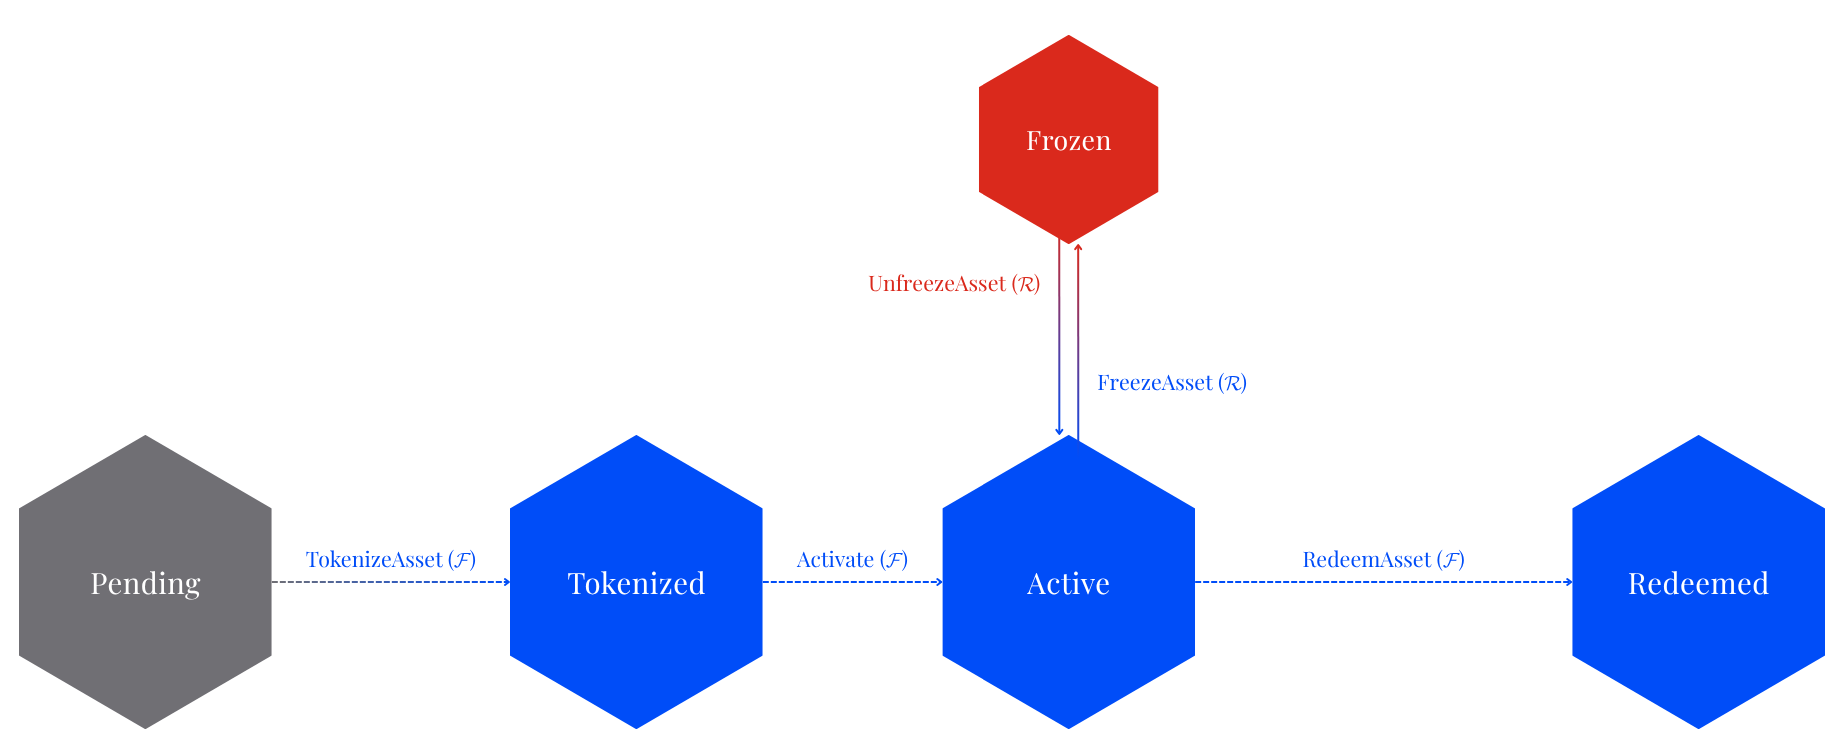
\includegraphics[width=\columnwidth]{figs/fig1.png}
\caption{Asset lifecycle state machine under the REC model.}
\label{fig:statemachine}
\end{figure}

% =========================================================
\section{Performance Evaluation}
\label{sec:perf}
% =========================================================

\subsection{Test Environment}

All projections are based on a simulation environment modeled after a reference Hyperledger Fabric deployment, parameterized as follows: three orderer nodes running EtcdRaft on dedicated virtual machines (8~vCPU, 32~GB RAM each); two endorsing peers (Peer~$\mathcal{F}$ and Peer~$\mathcal{R}$) on separate VMs (16~vCPU, 64~GB RAM); the smart contract environment co-located with Peer~$\mathcal{F}$; a graph database instance (4~vCPU, 16~GB RAM); and a 1~Gbps simulated LAN interconnect. Throughput projections are calibrated against the empirical Fabric performance characterization of Manevich \textit{et al.} \cite{ref:manevich}.

\subsection{Workload Definition}

Three workloads are defined to isolate the performance impact of each architectural layer. The baseline configuration employs a single-endorser ledger with only Peer~$\mathcal{F}$, without any off-chain AML check, executing a standard asset transfer invocation. The regulatory consensus configuration introduces the dual-endorser policy per $\mathbb{E}(\mathcal{T})$ while omitting the off-chain AML check, thereby isolating the cost of regulatory endorsement. The full analytical configuration adds an off-chain AML query per transaction to the dual-endorser setup, representing the complete production-equivalent stack.

\subsection{Projected Results}

The simulation-projected performance metrics are informed by prior Fabric benchmarks \cite{ref:manevich}. Under the baseline single-endorser configuration, the system achieves a mean throughput of 2,800~TPS (p99: 2,100~TPS) with a mean latency of 80\,ms (p99: 180\,ms). Introducing the dual-endorser policy decreases throughput to a mean of 1,350~TPS (p99: 950~TPS) with a mean latency of 180\,ms (p99: 320\,ms), reflecting the additional endorsement round-trip. Adding off-chain AML analysis further reduces throughput to a mean of 950~TPS (p99: 680~TPS) with a mean latency of 265\,ms (p99: 420\,ms). These figures represent estimated projections; empirical validation is identified as future work.

Even under the most demanding configuration, 950~TPS at a p99 latency of 420\,ms represents performance exceeding institutional RWA settlement requirements by two orders of magnitude: existing equity markets process approximately 10--15 transactions per second across settlement cycles measured in days \cite{ref:ecb_dlt}.

\subsection{Bottleneck Analysis}

The analysis reveals three primary bottlenecks in the architecture. The off-chain AML graph traversal introduces 50--100\,ms of latency per transaction, constituting the largest single overhead contributor in the full analytical configuration. The endorsement round-trip between Peer~$\mathcal{F}$ and Peer~$\mathcal{R}$ adds a mandatory network hop that contributes approximately 80\,ms under the simulated 1\,Gbps LAN. The endorsement policy complexity scales as $O(n)$ with the number of endorsing organizations $n$, as each additional bank or regulator increases gossip protocol overhead and endorsement collection time proportionally.

% =========================================================
\section{Threat Model and Security Analysis}
\label{sec:threat}
% =========================================================

We apply the STRIDE framework \cite{ref:stride} to the REC architecture, evaluating each threat category against the system's mitigations.

Identity spoofing is addressed through X.509 certificate-based authentication issued by organization-specific Certificate Authorities, with TLS mutual authentication enforced on all communication channels and securely managed credentials governing middleware-to-ledger interactions. Transaction tampering is rendered computationally infeasible by the hash-chained structure of the distributed ledger \cite{ref:fabric}, and any modification to smart contract logic requires re-deployment with a new version hash approved by the network's lifecycle endorsement policy. Repudiation is precluded by the dual-signature requirement of $\mathbb{E}(\mathcal{T})$, which ensures that every committed transaction carries the cryptographic endorsements of both $\mathcal{F}$ and $\mathcal{R}$, creating an immutable and non-repudiable audit trail with all MiCA threshold events additionally persisted on-ledger.

Information disclosure risks are mitigated by storing client PII and KYC documents off-chain in an encrypted database instance, with channel isolation preventing cross-organizational ledger reads; however, network-level traffic analysis could potentially reveal transaction timing patterns to a passive adversary. Denial of service constitutes the architecture's primary residual vulnerability, as a single-regulator deployment creates a liveness dependency whereby $\mathcal{R}$ going offline renders $\mathbb{E}(\mathcal{T})$ unsatisfiable and halts the network. A threshold signature scheme \cite{ref:threshold_sig} across multiple regulatory nodes would resolve this dependency. Elevation of privilege is prevented through cryptographic role separation, whereby only authorized identities registered under the regulatory provider can produce $\mathcal{R}$'s endorsement signature, and asset freezing and unfreezing functions enforce rigorous identity verification to reject non-regulatory invocations.

% =========================================================
\section{System Limitations and Risk Analysis}
\label{sec:limits}
% =========================================================

\subsection{Collusion Risk}

The security of the REC model relies on the adversarial independence of $\mathcal{F}$ and $\mathcal{R}$. The safety guarantee holds only when neither party is compromised by the other. If $\mathcal{F}$ and $\mathcal{R}$ collude, they jointly possess the cryptographic keys necessary to satisfy $\mathbb{E}(\mathcal{T})$ for arbitrary transactions, including non-compliant ones. Mitigation strategies include mandatory multi-regulator endorsement (requiring signatures from $|\mathcal{R}| \geq 2$ independent regulatory bodies) and cryptographic attestation of regulatory node software integrity via Trusted Execution Environments (TEEs) such as Intel SGX.

\subsection{Scalability vs. Decentralization}

The current deployment targets a minimal consortium (one bank, one regulator). Scaling to $n$ banks and $m$ regulators increases EtcdRaft ordering service complexity and endorsement policy evaluation time by $O(n + m)$. Furthermore, EtcdRaft's CFT model tolerates at most $\lfloor(n-1)/2\rfloor$ orderer failures; transitioning to a BFT ordering service (e.g., Mir-BFT \cite{ref:mirbft}) would be required for deployments with a larger, less trusted consortium.

\subsection{Off-Chain AML Oracle Dependency}

While the smart contract verifies syntactic ISIN and LEI correctness on-chain, semantic KYC/AML validation is delegated to the off-chain oracle. A compromised or bypassed middleware could allow a syntactically valid but semantically fraudulent transaction to reach the endorsement stage. Partially addressing this requires embedding a Merkle commitment to the AML check result within the transaction proposal, allowing the smart contract to verify that an AML check was performed without re-executing it on-chain. This pattern is analogous to zkSNARK-based compliance proofs \cite{ref:zksnark_compliance}.

\subsection{Governance Risks}

A single-regulator deployment creates a governance single point of failure. If $\mathcal{R}$'s infrastructure suffers an outage, the endorsement policy $\mathbb{E}(\mathcal{T})$ cannot be satisfied and the network halts, violating the liveness property. This is mitigated by deploying a quorum of regulatory nodes and using threshold signature schemes \cite{ref:threshold_sig}, such that $k$-of-$m$ regulatory signatures suffice to satisfy $\mathbb{E}(\mathcal{T})$, providing resilience against individual node failures.

\subsection{Cross-Jurisdictional Regulatory Conflicts}

In multi-national deployments, $\mathcal{R}$ may represent regulators from multiple jurisdictions (e.g., AMF~(France) and BaFin~(Germany)). Conflicting regulatory mandates, in which a transaction may be compliant under one jurisdiction's rules but not another's, create an endorsement deadlock. A dedicated governance protocol specifying conflict resolution procedures (e.g., majority-jurisdiction rule, escalation to a supranational authority such as ESMA) is required and represents a significant open problem at the intersection of blockchain governance and regulatory law.

% =========================================================
\section{Conclusion}
\label{sec:conclusion}
% =========================================================

The institutional tokenization of Real-World Assets requires a fundamental reconciliation between the cryptographic guarantees of distributed ledger technology and the non-negotiable mandates of financial regulation. Existing permissioned blockchain platforms fall short by relegating regulatory authorities to passive observers, creating a structural gap between on-chain execution and off-chain compliance.

In this paper, we introduced the Regulatory-Embedded Consensus (REC) model, a formally specified architecture built on Hyperledger Fabric that resolves this gap by elevating the regulatory authority to an active, cryptographically enforcing consensus participant. We proved that REC satisfies both safety and liveness under a non-colluding adversary model, formalized the architecture as a multi-layered theoretical system integrating smart contracts and off-chain analysis, and characterized its performance and security posture through simulation-based evaluation and STRIDE analysis.

Our simulation-based projections indicate that REC sustains 950--1,350~TPS at p99 latencies below 500\,ms, exceeding institutional RWA settlement requirements by two orders of magnitude. The principal limitations, namely collusion risk, AML oracle dependency, and single-regulator liveness, are explicitly characterized with concrete mitigation strategies as future work, including TEE-based regulatory node attestation, zkSNARK-based on-chain AML proof embedding, and threshold signature governance.

REC establishes a formal, implementable blueprint for the secure and compliant digitalization of global capital markets, bridging the gap between the programmability of blockchain and the accountability demanded by financial regulation.

% =========================================================
% Bibliography
% =========================================================
\bibliographystyle{IEEEtran}
\bibliography{refs}

\end{document}
